\documentclass[11pt]{article}
\usepackage[margin=0.9in]{geometry}
\usepackage[T1]{fontenc}
\usepackage{lmodern}
\usepackage{amsmath,amssymb,bm,booktabs,tabularx,array}
\usepackage{graphicx,float,microtype,fancyhdr}
\usepackage[hidelinks]{hyperref}
\usepackage{xurl}
\hypersetup{pdftitle={HPS-GPR v6.3: Reference matching and fixed-yield injections},pdfauthor={Emrys Peets}}
\pagestyle{fancy}\fancyhf{}\setlength{\headheight}{14pt}
\fancyhead[L]{\small HPS Gaussian-Process Resonance Search}
\fancyhead[R]{\small v6.3 / Injection design}\fancyfoot[C]{\thepage}
\fancypagestyle{plain}{\fancyhf{}\fancyhead[L]{\small HPS Gaussian-Process Resonance Search}
\fancyhead[R]{\small v6.3 / Injection design}\fancyfoot[C]{\thepage}}
\setlength{\emergencystretch}{2em}
\setlength{\parskip}{3pt}
\setlength{\tabcolsep}{6pt}
\renewcommand{\arraystretch}{1.14}
\newcommand{\E}{\mathbb E}
\newcommand{\Var}{\operatorname{Var}}
\newcommand{\Cov}{\operatorname{Cov}}
\newcommand{\Pois}{\operatorname{Poisson}}
\newcommand{\CV}{\operatorname{CV}}
\newcommand{\Ah}{\widehat A}
\newcommand{\sh}{\widehat\sigma}
\newcommand{\plain}[1]{\begin{quote}\textbf{In plain words.} #1\end{quote}}
\title{\vspace{-1em}HPS Gaussian-Process Resonance Search\\[.35em]
\large Reference Matching and Fixed-Yield Injections\\A short statistical study, v6.3}
\author{Emrys Peets}
\date{23 September 2026}
\begin{document}
\maketitle
\vspace{-.7em}

\section{Answer and the two questions being tested}
\textbf{Per-toy reference matching is statistically legitimate as a declared,
adaptive injection--recovery diagnostic.} It does not, by itself, test coverage
or detection power at one fixed physical signal yield. For that purpose, use
\textbf{one common expected yield per mass and dataset}, preferably chosen
from an independent background-only pilot sample and then frozen.
The existing matched study remains useful for understanding response and
signal absorption; changing the design does not automatically cure bias.

Let $B_t$ be background-only pseudoexperiment $t$, and define
\begin{equation}
 s_t=\sigma_{A,\mathrm{ref},t}=s(B_t),\qquad
 u_t=\Ah_t(0),\qquad e_t(A)=\sh_{A,t}(A).
 \label{eq:notation}
\end{equation}
Here $s_t$ is the fitted uncertainty on the \emph{signal yield} before adding
signal, $u_t$ is the signed zero-signal fitted yield, and $e_t(A)$ is the
uncertainty returned after injection. These are not a mass resolution or an
uncertainty on the ensemble mean. For $z\in\{1,3,5\}$, compare
\begin{equation}
 \boxed{A_t^{\mathrm M}=z\,s_t}\quad\hbox{(per-toy matched)},\qquad
 \boxed{A^{\mathrm F}=z\,s_0}\quad\hbox{(common expected yield)}.
 \label{eq:designs}
\end{equation}
In the proposed alternative, $s_0$ estimates the mean reference uncertainty
within a specified cell. $A$ denotes the \emph{expected} signal count; a
Poisson realization need not contain exactly $A$ signal candidates.

\plain{Matching gives a noisier toy a larger injected signal. A common yield
gives every toy the same expected number of signal candidates, allowing the
difficulty of extracting it to fluctuate naturally.}

\begin{table}[H]\centering
\begin{tabular}{rrrr}
\toprule
Input $z$ & Matched: $s_t=10$ & Matched: $s_t=20$ & Common: $s_0=15$\\
\midrule
1 & 10 & 20 & 15\\
3 & 30 & 60 & 45\\
5 & 50 & 100 & 75\\
\bottomrule
\end{tabular}
\caption{Illustrative yields in candidates, with the two reference errors equally
likely. Both designs have the same average yield, but different experiments.}
\end{table}

``Matched'' also means using the same binning, template, mask, fit procedure
and error convention for the reference and extraction. Keep that procedural
consistency in \emph{both} designs. It does not require $A$ to vary by toy.

\clearpage
\section{Why equal average yield does not make equal ensembles}
For this comparison, first take the ideal common scale $s_0=\E[s_t]$.
The mean injected yield agrees, but its variation does not:
\begin{align}
 \E[A_t^{\mathrm M}]&=A^{\mathrm F}=z s_0,&
 \Var(A_t^{\mathrm M})&=z^2\Var(s_t),&
 \Var(A^{\mathrm F})&=0,\\
 \frac{\operatorname{SD}(A_t^{\mathrm M})}{\E[A_t^{\mathrm M}]}&=\CV(s_t),&
 \frac{A_t^{\mathrm M}}{s_t}&=z,&
 \frac{A^{\mathrm F}}{s_t}&=z\frac{s_0}{s_t}.
 \label{eq:spread}
\end{align}
The last two ratios are nominal input strengths. Neither is automatically
the fitted significance, a discovery significance or a global significance.
An injected signal can alter the error and the fitted background.

Let $P_0$ generate the background and $K_A$ generate added signal counts at
expected yield $A$. The actual sampling laws are
\begin{align}
 P_{\mathrm M}(dB,dS)&=P_0(dB)\,K_{z s(B)}(dS),\\
 P_{\mathrm F}(dB,dS)&=P_0(dB)\,K_{z s_0}(dS).
 \label{eq:laws}
\end{align}
In the matched design, the signal expectation is a function of the same
background fluctuation that will be fitted. It is generally \emph{not} an
ordinary mixture of fixed-$A$ experiments: selecting a particular $s(B)$
also selects background realizations. If $s_t$ were constant, the two laws
would coincide. A small spread makes their input yields close, but does not
prove that nonlinear fit response or tail probabilities are equivalent.

\subsection*{Coverage and power have a fixed-parameter meaning}
For a confidence interval $I(Y)$ and a rejection rule $\phi(Y)$, the usual
quantities at fixed background nuisance parameters $\nu$ are
\begin{equation}
 C(A,\nu)=\Pr_{A,\nu}\{A\in I(Y)\},\qquad
 \pi(A,\nu)=\Pr_{A,\nu}\{\phi(Y)=1\}.
 \label{eq:coverage}
\end{equation}
The standard frequentist construction repeats the experiment at fixed
parameter values, generating the relevant auxiliary measurements as well
as the main data when they are part of the procedure~\cite{pdg}.
Matched-toy containment instead estimates
\begin{equation}
 C_{\mathrm M}=\Pr_{\mathrm M}\{z s(B)\in I(B+S)\}.
\end{equation}
This is a well-defined performance measure for the adaptive experiment.
It is not a measurement of $C(zs_0,\nu)$.

\plain{For a coverage claim, the truth must stay put while the experiment
fluctuates. If the truth moves with each toy, a containment fraction answers
a different question.}

This distinction does not imply that matched pulls \emph{must} fail. In an
ideal location model $\Ah=A+s_t E_t$ with $E_t\sim N(0,1)$ independent of
$s_t$ and a correctly returned error $s_t$, the pull is $E_t$ for either
design. Matching neither forces a biased estimator to close nor proves
fixed-yield performance when closure is observed.

\clearpage
\section{Separate background offset, signal response and error calibration}
To expose the mechanism, write the local conditional-mean response as
\begin{equation}
 \E[\Ah_t(A)\mid B_t]=u_t+g_t A+O(A^2).
 \label{eq:linear}
\end{equation}
The signal draw is averaged on the left. $u_t$ is the background-dependent
offset; $g_t=1$ means unit incremental response and $g_t<1$ means a loss of
injected yield in this approximation. Ignoring the displayed nonlinear term,
the ensemble mean biases are
\begin{align}
 b_{\mathrm M}&=\E[u_t]+z\E[(g_t-1)s_t],\\
 b_{\mathrm F}&=\E[u_t]+z s_0(\E[g_t]-1),\\
 \boxed{b_{\mathrm M}-b_{\mathrm F}=z\Cov(g_t,s_t)}&\qquad (s_0=\E[s_t]).
 \label{eq:covbias}
\end{align}
Thus a correlation between sensitivity and absorption changes the average
bias even when the mean injected yield agrees. The coefficient of variation
of $s_t$ alone cannot determine that correlation.

\subsection*{Three quantities that should be reported together}
For $A_t>0$, define the raw recovery, paired response and pull as
\begin{equation}
 Q_t=\frac{\Ah_t(A_t)}{A_t},\qquad
 R_t=\frac{\Ah_t(A_t)-\Ah_t(0)}{A_t},\qquad
 p_t=\frac{\Ah_t(A_t)-A_t}{e_t(A_t)}.
 \label{eq:metrics}
\end{equation}
Raw recovery includes the background offset. The paired response subtracts
that offset to isolate the response to adding signal. In the linear model,
$\E[R_t\mid B_t]=g_t$ in either design; an individual Poisson signal draw
makes $R_t$ noisy. A raw average of $Q_t$ additionally contains
$\E[u_t/s_t]/z$ under matching, or $\E[u_t]/(zs_0)$ at common yield.
Even $\E[u_t]=0$ does not imply $\E[u_t/s_t]=0$.

Do not interchange the average of per-toy ratios and the ratio of averages.
For matched injections in this linear model,
\begin{equation}
 \E[R_t]=\E[g_t],\qquad
 \frac{\E[\Ah_t(A_t)-\Ah_t(0)]}{\E[A_t]}
 =\frac{\E[g_t s_t]}{\E[s_t]}
 =\E[g_t]+\frac{\Cov(g_t,s_t)}{\E[s_t]}.
\end{equation}

\begin{table}[H]\centering\small
\begin{tabular}{lrrrr}
\toprule
Design & Mean $A$ & Mean bias & Mean $Q_t$ & Mean $R_t$\\
\midrule
Per-toy matched & 45 & $-6.30$ & 0.923 & 0.890\\
Common yield & 45 & $-4.95$ & 0.890 & 0.890\\
\bottomrule
\end{tabular}
\caption{Exact illustrative example at $z=3$: equally likely states have
$s=(10,20)$, $u=(4,-4)$ and $g=(0.98,0.80)$. Bias is in candidates.
The difference is $3\Cov(g,s)=-1.35$. These are not HPS measurements.}
\end{table}

Always use each injected fit's returned error in the pull; replacing it by
the pilot mean would test a different error prescription. Pull moments are
diagnostics, not substitutes for interval coverage. For physical inference,
retain the raw fitted yield; paired subtraction is a response diagnostic.

\textbf{At $z=0$ both designs inject zero.} With the same background draws
and fitting procedure, their null distributions are identical. Changing
injection scaling cannot remove a null offset. Also distinguish a signed
local estimator from a positive, one-sided scan maximum; v5.9.5 addresses
these separately~\cite{nullstudy}.

\clearpage
\section{What the archived HPS implementation actually did}
The v5.0.5 methodology defines a zero-signal reference fit for each source,
toy and mass, followed by $A_t=z\sigma_{A,\mathrm{ref},t}$ and a refit of
the injected spectrum~\cite{note}. The audit for this report follows the
preserved v4.6 full-100 baseline used in the note's consolidated validation
displays. It covers four 2021 exposure/source constructions and five masses
(65, 90, 120, 180, 210~MeV), with 7,994 accepted extraction rows.
It does not pool the later targeted threshold replacements.

The saved rows and generating code establish the following:
\begin{itemize}
 \item The actual injection scale is the selected background-only fit's
 returned \texttt{sigma\_A}, saved as \texttt{sigmaA\_ref}. The reference
 fit uses that toy's fluctuated counts, including its held-out extraction
 region. It is not a universal Asimov scale.
 \item All 5,995 accepted positive-injection rows satisfy
 $A_t=z s_t$, to an absolute numerical residual below
 $3\times10^{-11}$ candidates. Their saved reference error equals the
 corresponding zero-injection returned error exactly.
 \item Added signal counts are \textbf{Poisson fluctuated}. Across the
 accepted rows, $(N_{\mathrm{sig}}-A_t)/\sqrt{A_t}$ has descriptive sample
 standard deviation 1.005. The code, rather than this pooled check alone,
 establishes the sampling mode.
\end{itemize}

\begin{table}[H]\centering\small
\begin{tabular}{rrrrr}
\toprule
Mass [MeV] & Mean $s_t$ & SD$(s_t)$ & CV [\%] & $\operatorname{Corr}(s_t,u_t)$\\
\midrule
65 & 7,327.5 & 206.2 & 2.814 & +0.162\\
90 & 6,494.3 & 154.4 & 2.377 & -0.344\\
120 & 5,055.3 & 90.7 & 1.794 & -0.065\\
180 & 2,853.6 & 53.9 & 1.890 & +0.079\\
210 & 2,144.0 & 43.5 & 2.027 & +0.180\\
\bottomrule
\end{tabular}

\caption{Historical 2021 10\% baseline, 100 reference toys per mass. Errors
and their standard deviations are in signal candidates. CV is
$\operatorname{SD}(s_t)/\overline s$. The last column is the descriptive
sample correlation with the signed zero-injection yield. It is not a
significance test.}
\label{tab:archive}
\end{table}

Across all 20 historical cells, the CV ranges from 1.17\% to 3.00\%.
Consequently, the matched \emph{expected} yields vary by that relative
amount; this excludes the additional Poisson variation of actual signal
counts. At 65~MeV in the 2021 10\% row, a common scale equal to the saved
mean would give approximately 7,327, 21,982 and 36,637 expected candidates
at $z=1,3,5$. These are illustrative translations of an existing ensemble,
not new fixed-yield fit results.

\plain{In this archived baseline the two injection choices are numerically
quite close in yield. The audit does not show that reference matching caused
the observed bias, and it cannot reconstruct how new fixed-yield fits would
behave.}

There are two naming traps. On zero-injection rows,
\texttt{sigmaA\_reference} is a \emph{separate Asimov diagnostic}; using that
column would audit the wrong quantity. Also, the older v4.6 plotting code
labels $\Ah/A_{\mathrm{inj}}$ as recovery, whereas the v5.0.5 methodology
defines the paired response in Eq.~\eqref{eq:metrics}. The audit preserves
and computes both definitions without relabeling historical plots.

\clearpage
\section{How to choose the common reference uncertainty}
For a fixed dataset, mass, template and fit prescription, use an independent
pilot ensemble of $M$ background-only fits:
\begin{equation}
 s_0=\overline s_{\mathrm{pilot}}=\frac1M\sum_{j=1}^{M}s_j^{\mathrm{pilot}},
 \qquad A\in\{0,s_0,3s_0,5s_0\}.
 \label{eq:pilot}
\end{equation}
Freeze that value before generating the evaluation toys. Conditional on the
frozen pilot result, every evaluation toy then has the same expected signal
yield. Pilot precision is approximately
\begin{equation}
 \frac{\operatorname{SE}(\overline s_{\mathrm{pilot}})}{\E[s]}
 \simeq\frac{\CV(s)}{\sqrt M}.
\end{equation}
This quantifies precision of the chosen injection coordinate; it does not
include uncertainty in the physical background truth.

A mean over the \emph{same} evaluation backgrounds is usable as an exploratory
common-yield check, but retains a weak dependence on those backgrounds.
For independent, identically distributed background toys and a baseline
statistic $u_t=u(B_t)$,
\begin{equation}
 \Cov\!\left(z\overline s_T,u_t\right)
 =\frac{z}{T}\Cov(s_t,u_t).
 \label{eq:reuse}
\end{equation}
It shrinks with ensemble size, unlike the per-toy dependence
$\Cov(zs_t,u_t)=z\Cov(s_t,u_t)$. The independent pilot removes this
particular dependence; it is the cleaner design for a fixed-yield test.

\begin{figure}[H]\centering
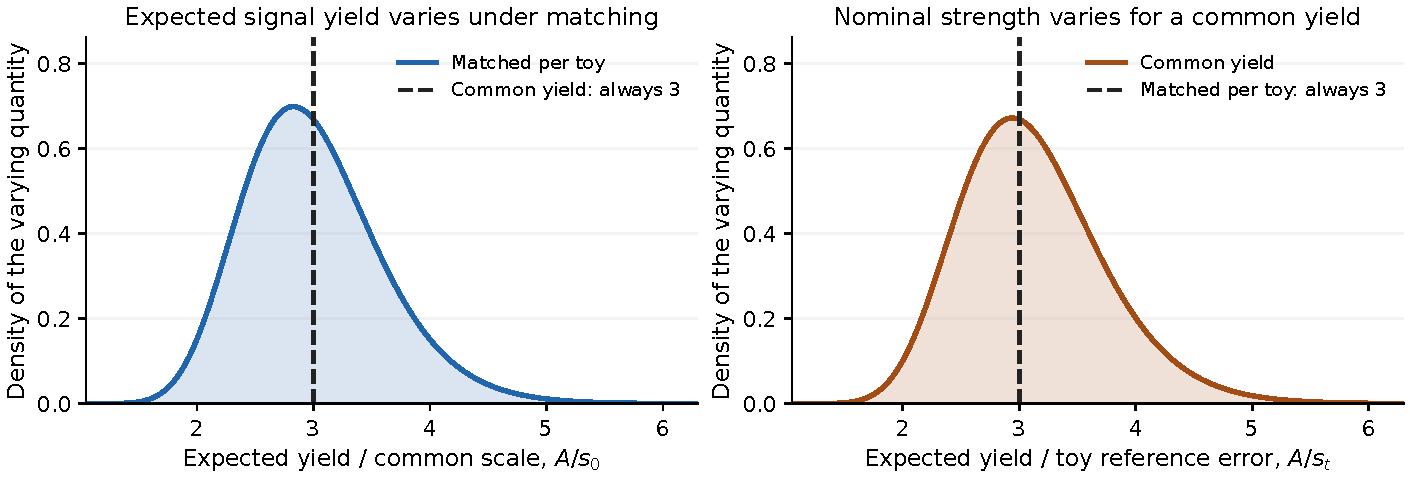
\includegraphics[width=\linewidth]{../figures/injection_design.pdf}
\caption{Analytic illustration at $z=3$, with a positive lognormal reference
error having mean $s_0$ and CV 20\%. The broad spread is chosen for visibility
and is \emph{not} the measured HPS spread. Curves are densities of the varying
quantity; dashed lines mark a constant value, not a density height. Matching
fixes $A/s_t$ and varies $A$; a common yield fixes $A$ and varies $A/s_t$.}
\end{figure}

An Asimov background-only fit also supplies a common scale; its curvature
error need not equal the mean error of fluctuated fits~\cite{cowan}. For a
target median local significance, tune a fixed $A$ with the Asimov
approximation and verify it with toys. $A/s_0$ alone need not equal that
significance.

The mean error differs from both $\sqrt{\E[s_t^2]}$ and
$\operatorname{SD}(\Ah_t(0))$. The last measures estimator variation;
averaging errors does not establish their calibration. Do not pool masses,
datasets or incompatible yield normalizations. To compare extraction
methods, use one nominal scale and the \emph{same injected spectra}.

\clearpage
\section{A separate choice: fluctuate the number of signal candidates}
Choosing a common $A$ does \emph{not} require adding exactly $A$ candidates
to every toy. Let $w_i$ be full-template signal probabilities and include
out-of-support categories so that $\sum_i w_i=1$. Let
$B_i\sim\Pois(b_i)$ independently. Three useful designs have different
sampling variances:

\begin{table}[H]\centering\small
\begin{tabularx}{\linewidth}{@{}l >{\raggedright\arraybackslash}X >{\raggedright\arraybackslash}X@{}}
\toprule
Signal construction & Mean and covariance & Question it addresses\\
\midrule
Deterministic template &
$S_i=A w_i$, $\Cov(S)=0$ &
Mean-response and absorption control; omits signal counting noise.\\[4pt]
Exactly $N$ candidates &
$S\sim\operatorname{Multinomial}(N,\bm w)$;
$\E[S]=N\bm w$,
$\Cov(S)=N[\operatorname{diag}(\bm w)-\bm w\bm w^T]$ &
Recovery of a specified injected sample size; the total count is fixed.\\[4pt]
Poisson signal yield &
$S_i\sim\Pois(Aw_i)$ independently;
$\Cov(S)=A\operatorname{diag}(\bm w)$ &
Repeated counting experiments at a fixed expected signal rate $A$.\\
\bottomrule
\end{tabularx}
\caption{The background counting covariance adds to these covariances when
the fixed-yield signal draw is independent of the background. For matched
injections these signal formulas apply conditional on $B$; marginally the
adaptive dependence must also be retained.}
\end{table}

Drawing $N_{\mathrm{sig}}\sim\Pois(A)$ and then placing those candidates
multinomially is equivalent to independent binwise Poisson draws. In the
fixed-yield rate experiment,
\begin{equation}
 B_i+S_i\sim\Pois(b_i+A w_i).
 \label{eq:poisson}
\end{equation}
By contrast, an exactly-$N$ signal has negative cross-bin covariances and
no fluctuation in its total. Deterministic addition has no signal counting
variance at all. A Poisson extraction likelihood applied to these other
ensembles need not produce unit pull widths or nominal interval coverage,
even with the correct background mean.

\plain{``Inject the same signal'' should usually mean the same expected
rate. Real counting experiments fluctuate around that rate. Adding exactly
the same number of candidates is a useful controlled experiment, but it
removes one source of fluctuation.}

For Poisson signal under per-toy matching, total signal variance satisfies
\begin{equation}
 \Var(N_{\mathrm{sig}})=\E[A_t]+\Var(A_t)
 =z\E[s_t]+z^2\Var(s_t).
\end{equation}
At a common expected yield it is just $A$. The extra term is variation of
the chosen truth between toys; it is not an additional detector uncertainty.
Pulls must subtract each toy's own expected $A_t$, not an ensemble average
or that toy's realized $N_{\mathrm{sig}}$, when assessing a Poisson-rate
estimator.

\subsection*{Relation to v6.2}
The current v6.2 MC study already uses common sample sizes
$N=1{,}000,5{,}000,10{,}000,30{,}000$ at each mass, with exactly-$N$
multinomial signal and Poisson background~\cite{mcstudy}. It is a fixed-count
recovery study, rather than a new per-toy reference-matched scan. Its GP
conditional mean and covariance are recomputed, while archived kernel
hyperparameters remain fixed. For a Poisson-rate coverage follow-up, keep a
common \emph{expected} $A$ and also fluctuate the total signal count. In
either case, repeat whichever fit procedure the claimed result actually uses.

\clearpage
\section{Recommended next test and what this report establishes}
\begin{enumerate}
 \item \textbf{Define the cell and yield.} Fix dataset, mass, full signal
 template, generating background and extraction prescription. Preserve the
 production $\pm2.25\sigma_m$ exclusion window. State whether $A$ is a
 full selected yield or a yield restricted to a specified region.
 \item \textbf{Freeze a common scale.} Use an independent background-only
 pilot mean, or a declared Asimov scale, then take
 $A=0,s_0,3s_0,5s_0$. Use the same absolute yields when comparing methods
 or testing robustness to alternative generating backgrounds; give any
 separate equal-difficulty comparison its own label.
 \item \textbf{Generate evaluation toys.} For rate inference draw independent
 Poisson background and signal counts. Sharing each background across
 injection levels provides useful paired controls. Fit identical spectra
 with competing methods; account for the pairing when estimating differences.
 \item \textbf{Keep the three diagnostics.} Report signed raw bias,
 per-fit-error pulls, and paired incremental response. Report failed fits
 and their selection rule. Do not discard statistical outliers or tune a
 bias correction on the evaluation sample.
 \item \textbf{Measure coverage or power separately.} At each fixed $A$,
 evaluate the actual interval construction or test, with binomial uncertainty
 on the resulting fraction. Repeating a fitted, frozen background source
 gives a source-conditional result; it does not establish uniform performance
 over unknown physical backgrounds. Keep the matched design as a secondary
 response check.
\end{enumerate}

\textbf{Decision.} The proposed average-error injection is a sensible primary
design for a common-yield validation, with an independent pilot as the clean
implementation. There is no basis here to discard the older matched study
as statistically invalid. It asks a different question, and the archived
baseline has only a few percent variation in its matched expected yields.
Neither design alone validates the physical background or fixes null bias.

\subsection*{Scope, audit trail and reproduction}
This study derives the comparison and audits archived rows; it runs
\textbf{no new HPS fits} and estimates no new coverage or discovery
probability. The package includes LaTeX, the analytic figure, minimal
archived rows, scripts, CSVs and SHA-256 provenance. Run
\texttt{bash reproduce.sh}; see \texttt{README.md} for tool paths.
The original row source has SHA-256 prefix \texttt{b23f31975b50};
\texttt{audit/} contains full hashes and line evidence. Later threshold
replacements are outside this quantitative audit.

\begin{thebibliography}{9}\small\setlength{\itemsep}{2pt}\setlength{\parskip}{0pt}
\bibitem{pdg} G.~Cowan and L.~Lista, ``Statistics,'' \emph{Review of Particle
Physics} (2026), especially Secs.~40.2.6.1 and 40.4.2.
\href{https://pdg.lbl.gov/2026/reviews/rpp2026-rev-statistics.pdf}{PDG Statistics review}.
\bibitem{cowan} G.~Cowan, K.~Cranmer, E.~Gross and O.~Vitells,
``Asymptotic formulae for likelihood-based tests of new physics,''
\emph{Eur. Phys. J. C} \textbf{71}, 1554 (2011), Secs.~3.2 and 4.1.
\href{https://arxiv.org/abs/1007.1727}{arXiv:1007.1727}.
\bibitem{note} HPS-GPR analysis note v5.0.5 (16 September 2026),
``Matched-reference injection--extraction diagnostics'' and
``Matched refits and fit-quality checks.'' Preserved v4.6 full-100 baseline
code and accepted rows are identified in the accompanying audit.
\bibitem{nullstudy} HPS-GPR v5.9.5, \emph{Apparent null bias}
(22 September 2026), local study package.
\bibitem{mcstudy} HPS-GPR v6.2, \emph{Reconstructed-MC injection and signal
recovery} (23 September 2026), local study package, 40-toy release.
\end{thebibliography}
\end{document}
